
\documentclass[letterpaper, 10pt, conference]{ieeeconf}
\usepackage{graphicx}
\overrideIEEEmargins
\usepackage[utf8]{inputenc}
\usepackage[T1]{fontenc}
\usepackage{graphics}
\usepackage{amsmath}
\usepackage{amssymb}
\usepackage{booktabs}

% Spanish names and arabic numbering for tables (figures already use Fig. in ieeeconf)
\makeatletter
\renewcommand{\fnum@table}{Tabla~\thetable.}
\makeatother
\renewcommand{\thetable}{\arabic{table}}

\title{\LARGE \bf
Clasificaci\'on de Sentimientos de Rese\~nas de Pel\'iculas en IMDb\\
con Redes Neuronales Recurrentes
}

\author{
  Yezid Garcia$^{*}$, Juan Martin Santos$^{*}$, Jaime Rodriguez$^{*}$ \\
  $^{*}$Grupo 24. C\'odigos: 200810710, 202013610, 200717791
}

\begin{document}

\maketitle
\thispagestyle{empty}
\pagestyle{empty}

%%%%%%%%%%%%%%%%%%%%%%%%%%%%%%%%%%%%%%%%%%%%%%%%%%%%%%%%%%%%%%%%%%%%%%%%%%%%%%%%
\section{Introducci\'on}

El an\'alisis de sentimiento es una tarea del procesamiento de lenguaje natural
que determina la polaridad emocional de un texto. En el contexto de rese\~nas
de pel\'iculas, el problema se reduce a clasificaci\'on binaria: identificar si
una rese\~na expresa una opini\'on positiva o negativa. Su aplicaci\'on permite
caracterizar la opini\'on del p\'ublico de forma autom\'atica, con utilidad en
sistemas de recomendaci\'on y monitoreo de reputaci\'on.

Los enfoques cl\'asicos basados en frecuencia de t\'erminos ignoran el orden de
las palabras y pierden informaci\'on contextual. Las redes con celdas de memoria
a largo y corto plazo (LSTM) [1] superan esta limitaci\'on al procesar
secuencias de tokens y capturar dependencias entre palabras distantes. La
variante bidireccional (BiLSTM) combina estados ocultos en ambas direcciones,
proporcionando a cada posici\'on acceso al contexto anterior y posterior. Las
representaciones distribucionales de palabras [2] codifican similitud
sem\'antica en vectores densos entrenados sobre grandes corpus; inicializar un
modelo con vectores preentrenados como GloVe [3] mejora la generalizaci\'on
cuando el conjunto de entrenamiento es de tama\~no moderado.

Este trabajo presenta la implementaci\'on y evaluaci\'on de un modelo BiLSTM
con embeddings GloVe para la clasificaci\'on binaria de rese\~nas del conjunto
IMDb [4]. Se describe el pipeline de preprocesamiento, la arquitectura del
modelo, la estrategia de entrenamiento y los resultados obtenidos en t\'erminos
de precisi\'on, recall y F1-score.

%%%%%%%%%%%%%%%%%%%%%%%%%%%%%%%%%%%%%%%%%%%%%%%%%%%%%%%%%%%%%%%%%%%%%%%%%%%%%%%%
\section{Metodolog\'ia}

El conjunto de datos contiene 40\,000 rese\~nas de IMDb [4] con etiqueta
binaria de sentimiento, balanceado en 20\,000 muestras por clase y sin valores
nulos. La partici\'on es estratificada: 80\,\% para entrenamiento (32\,000
muestras), 10\,\% para validaci\'on (4\,000) y 10\,\% para prueba (4\,000).

Cada rese\~na pasa por un pipeline de preprocesamiento de cinco pasos:
eliminaci\'on de etiquetas HTML; descarte de caracteres no alfab\'eticos;
conversi\'on a min\'usculas; eliminaci\'on de palabras funcionales en ingl\'es;
y lematizaci\'on, que reduce cada token a su forma can\'onica (por ejemplo,
\textit{running} a \textit{run}). Los tokens resultantes se convierten a
\'indices enteros usando un vocabulario construido exclusivamente sobre el
conjunto de entrenamiento, y las secuencias se rellenan o truncan a 300 tokens.

Los embeddings se inicializan con vectores GloVe de 100 dimensiones [3]; la
cobertura sobre el vocabulario del conjunto es del 77.2\,\%. Siguiendo la
estrategia de ajuste progresivo propuesta en [5], los embeddings se congelan
durante las tres primeras \'epocas para que las capas recurrentes converjan sin
distorsionar las representaciones preentrenadas. A partir de la cuarta \'epoca,
se descongelan con una tasa de aprendizaje diez veces menor para realizar un
ajuste fino controlado.

El modelo, denominado \textit{SentimentBiLSTM}, combina cuatro etapas descritas
en la Tabla 1. Una capa BiLSTM de 128 unidades por direcci\'on procesa la
secuencia en ambos sentidos; luego un promedio sobre todos los estados ocultos
(mean pooling) produce una representaci\'on de longitud fija. Esta operaci\'on,
validada en [6], es superior al uso del \'ultimo estado oculto para secuencias
largas donde el sentimiento est\'a distribuido a lo largo del texto. Una capa
lineal con activaci\'on sigmoide clasifica en positivo o negativo.

\begin{table}[h]
\centering
\caption{Capas del modelo \textit{SentimentBiLSTM}.}
\label{tab:arquitectura}
\resizebox{8.5cm}{!}{
\begin{tabular}{llr}
\toprule
\textbf{Capa} & \textbf{Dimensi\'on de salida} & \textbf{Par\'ametros} \\
\midrule
Embedding GloVe 100d      & $B \times 300 \times 100$ & 7{,}449{,}500 \\
Abandono (p = 0.3)        & $B \times 300 \times 100$ & 0             \\
BiLSTM (128 ud., 1 capa)  & $B \times 300 \times 256$ & 267{,}264     \\
Mean Pooling              & $B \times 256$            & 0             \\
Abandono (p = 0.3)        & $B \times 256$            & 0             \\
Lineal + Sigmoide         & $B \times 1$              & 257           \\
\midrule
\textbf{Total}            &                           & \textbf{7{,}685{,}277} \\
\bottomrule
\end{tabular}}
\end{table}

El entrenamiento usa el optimizador Adam con tasa de aprendizaje inicial de
$10^{-3}$ y p\'erdida de entrop\'ia cruzada binaria, con lotes de 128 muestras.
Se incorporan tres mecanismos de control: un planificador que reduce la tasa de
aprendizaje a la mitad si la p\'erdida de validaci\'on no mejora en dos
\'epocas consecutivas; limitaci\'on de la norma del gradiente a 1.0, que [7] identifica como
cr\'itico para estabilizar LSTM en secuencias largas; y parada anticipada con paciencia de cinco \'epocas. Las m\'etricas de
evaluaci\'on son precisi\'on, recall y F1-score.

%%%%%%%%%%%%%%%%%%%%%%%%%%%%%%%%%%%%%%%%%%%%%%%%%%%%%%%%%%%%%%%%%%%%%%%%%%%%%%%%
\section{Resultados}

\subsection{Resultados cuantitativos}

Se entren\'o el modelo durante un m\'aximo de 20 \'epocas; la parada anticipada
se activ\'o en la \'epoca 19. La Fig. 1 muestra la evoluci\'on de la p\'erdida
y las m\'etricas de validaci\'on a lo largo del entrenamiento.

\begin{figure}[h]
  \centering
  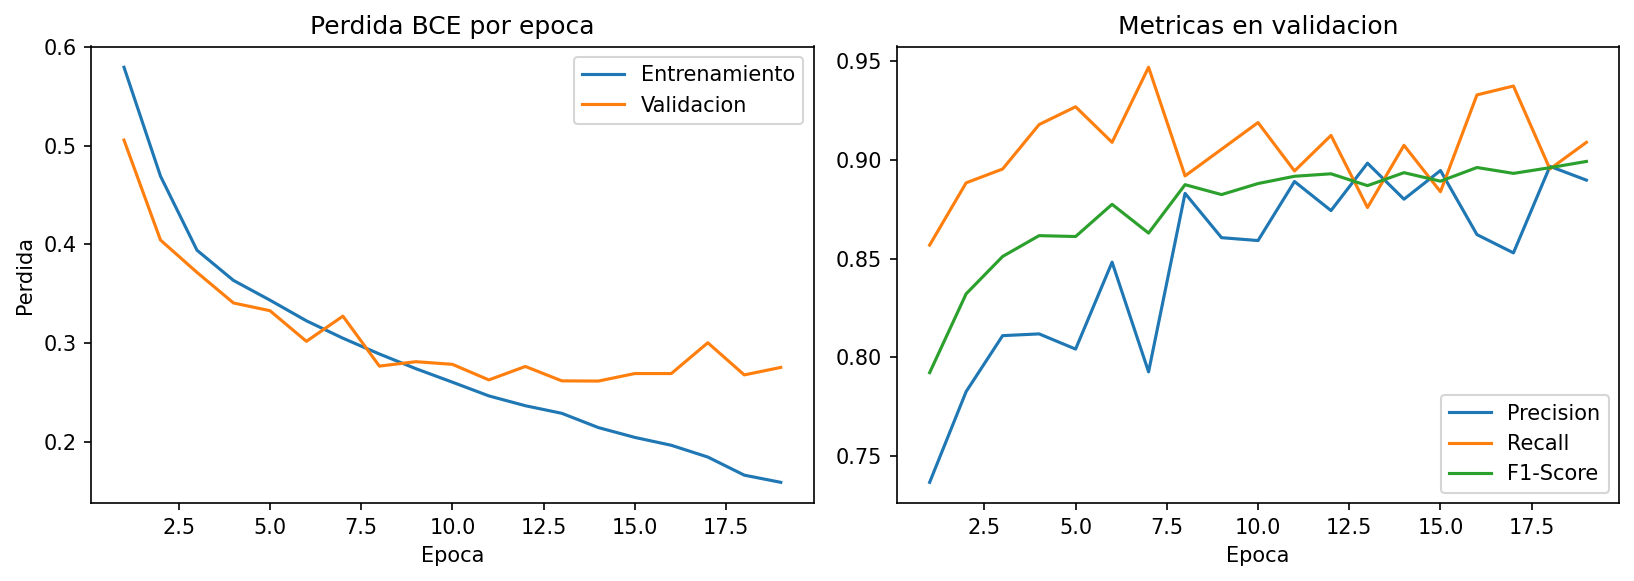
\includegraphics[width=0.98\linewidth]{curvas_entrenamiento.png}
  \caption{P\'erdida BCE (izq.) y m\'etricas de validaci\'on (der.) por
  \'epoca. La parada anticipada se activa en la \'epoca 19.}
  \label{fig:curvas}
\end{figure}

La Tabla 2 compara las m\'etricas en tres momentos clave para mostrar el efecto
de la estrategia de ajuste progresivo: al terminar la fase de congelado (\'ep.
3), al inicio del ajuste fino (\'ep. 6) y al final del entrenamiento (\'ep. 19).
La Tabla 3 reporta los resultados sobre el conjunto de prueba.

\begin{table}[h]
\centering
\caption{Evoluci\'on de m\'etricas en validaci\'on por fase.}
\label{tab:evolucion}
\resizebox{8.5cm}{!}{
\begin{tabular}{lccc}
\toprule
\textbf{Fase} & \textbf{Precisi\'on} & \textbf{Recall} & \textbf{F1} \\
\midrule
\'Ep. 3 --- embeddings congelados   & 0.811 & 0.895 & 0.851 \\
\'Ep. 6 --- inicio ajuste fino      & 0.848 & 0.909 & 0.878 \\
\'Ep. 11 --- convergencia           & 0.889 & 0.894 & 0.892 \\
\'Ep. 19 --- parada anticipada      & 0.890 & 0.909 & 0.899 \\
\bottomrule
\end{tabular}}
\end{table}

\begin{table}[h]
\centering
\caption{M\'etricas finales sobre el conjunto de prueba.}
\label{tab:prueba}
\begin{tabular}{lc}
\toprule
\textbf{M\'etrica} & \textbf{Valor} \\
\midrule
Precisi\'on  & 0.877 \\
Recall       & 0.910 \\
F1-Score     & \textbf{0.893} \\
\bottomrule
\end{tabular}
\end{table}

\subsection{Resultados cualitativos}

El recall supera sistem\'aticamente a la precisi\'on tanto en validaci\'on como
en prueba (0.910 frente a 0.877), lo que indica una tendencia del modelo a
clasificar como positivo ante la ambig\"uedad. Esto es consistente con el sesgo
de los vectores GloVe: intensificadores frecuentes en rese\~nas como
\textit{amazing} o \textit{terrible} tienen carga emocional pronunciada que el
modelo asocia con la clase positiva incluso en contextos negativos. El efecto
persiste tras el ajuste fino.

La convergencia es r\'apida en las primeras seis \'epocas, donde el F1 pasa
de 0.792 a 0.878; las \'epocas siguientes aportan mejoras marginales. La
brecha creciente entre p\'erdida de entrenamiento y validaci\'on a partir de
la \'epoca 11 se\~nala sobreajuste moderado que la parada anticipada contiene
pero no elimina.

%%%%%%%%%%%%%%%%%%%%%%%%%%%%%%%%%%%%%%%%%%%%%%%%%%%%%%%%%%%%%%%%%%%%%%%%%%%%%%%%
\section{Discusi\'on}

El F1 de 0.893 es consistente con los rangos reportados en trabajos sobre IMDb
con arquitecturas recurrentes [5]. El resultado se ubica en el rango esperado
para una sola capa BiLSTM, ya que [7] muestra que arquitecturas m\'as profundas
no siempre mejoran el rendimiento en tareas de clasificaci\'on de longitud
moderada y pueden introducir inestabilidad en el entrenamiento. El mean pooling
sobre los estados ocultos, respaldado por [6], produce representaciones m\'as
robustas que el \'ultimo estado oculto en rese\~nas largas donde el sentimiento
est\'a distribuido a lo largo del texto, lo que explica la estabilidad de las
m\'etricas en las \'epocas finales.

La estrategia de congelar y luego descongelar los embeddings es efectiva: la
Tabla 2 muestra una ganancia de 2.7 puntos de F1 entre la \'epoca 3 y la
\'epoca 6, en l\'inea con los resultados de [2] al comparar estrategias de
embeddings est\'aticos y ajustables. El ajuste fino con tasa de aprendizaje
reducida evita destruir las representaciones preentrenadas mientras el modelo
captura patrones espec\'ificos del dominio. La cobertura del 77.2\,\% de GloVe
sobre el vocabulario del conjunto es suficiente para que los embeddings aporten
informaci\'on sem\'antica \'util desde las primeras \'epocas.

Como limitaciones, el n\'umero de \'epocas de congelado es fijo, por lo que
un criterio adaptativo podr\'ia ajustarse mejor seg\'un la velocidad de
convergencia de cada ejecuci\'on. Las rese\~nas con m\'as de 300 tokens se
truncan, perdiendo el contexto del final del texto, que en cr\'iticas de cine
frecuentemente contiene la valoraci\'on final del autor. Tampoco se realiz\'o
b\'usqueda sistem\'atica de hiperpar\'ametros, por lo que la configuraci\'on
actual puede no ser \'optima. Como trabajo futuro, resulta de inter\'es
explorar mecanismos de atenci\'on sobre los estados del BiLSTM como alternativa
al mean pooling, comparar el rendimiento con un codificador Transformer ligero
y evaluar el impacto de distintas duraciones de la fase de congelado.

%%%%%%%%%%%%%%%%%%%%%%%%%%%%%%%%%%%%%%%%%%%%%%%%%%%%%%%%%%%%%%%%%%%%%%%%%%%%%%%%
\clearpage

\begin{thebibliography}{99}

\bibitem{hochreiter1997}
S.~Hochreiter and J.~Schmidhuber,
``Long short-term memory,''
\textit{Neural Computation}, vol.~9, no.~8, pp.~1735--1780, 1997.

\bibitem{kim2014}
Y.~Kim,
``Convolutional neural networks for sentence classification,''
in \textit{Proc. EMNLP}, pp.~1746--1751, 2014.

\bibitem{pennington2014}
J.~Pennington, R.~Socher, and C.~D.~Manning,
``GloVe: Global vectors for word representation,''
in \textit{Proc. EMNLP}, pp.~1532--1543, 2014.

\bibitem{maas2011}
A.~L.~Maas, R.~E.~Daly, P.~T.~Pham, D.~Huang, A.~Y.~Ng, and C.~Potts,
``Learning word vectors for sentiment analysis,''
in \textit{Proc. 49th Annual Meeting of the ACL}, pp.~142--150, 2011.

\bibitem{howard2018}
J.~Howard and S.~Ruder,
``Universal language model fine-tuning for text classification,''
in \textit{Proc. ACL}, pp.~328--339, 2018.

\bibitem{conneau2017}
A.~Conneau, D.~Kiela, H.~Schwenk, L.~Barrault, and A.~Bordes,
``Supervised learning of universal sentence representations from natural
language inference data,''
in \textit{Proc. EMNLP}, pp.~670--680, 2017.

\bibitem{greff2015}
K.~Greff, R.~K.~Srivastava, J.~Kout\'nik, B.~R.~Steunebrink, and J.~Schmidhuber,
``LSTM: A search space odyssey,''
\textit{IEEE Trans. Neural Netw. Learn. Syst.}, vol.~28, no.~10,
pp.~2222--2232, 2017.

\bibitem{mikolov2013}
T.~Mikolov, K.~Chen, G.~Corrado, and J.~Dean,
``Efficient estimation of word representations in vector space,''
\textit{arXiv preprint arXiv:1301.3781}, 2013.

\end{thebibliography}

\end{document}
